\documentclass[12pt,fleqn]{article}\usepackage{../../common}
\begin{document}
Modern Bilim Öncesi Bilimsel, Astronomik Buluşlar, Gezegenler, Yörüngeler

Dünya - Ay Mesafe Oranı

Aristarchus dünya-güneş ve dünya-ay mesafeleri arasında bir oran hesaplamayı
başardı [1]. Bunu yapmak için basit açılar kullanması yeterli oldu. Önce ayın
yarım ay fazına gelmesini bekledi,

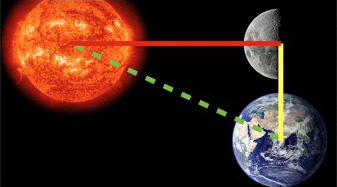
\includegraphics[width=20em]{moonshad.jpg}

Bu durumda güneş-ay-dünyanın birbirine belli bir şekilde duracağını biliyordu, ki
bu ilişki alttaki gibi çizilebilir,

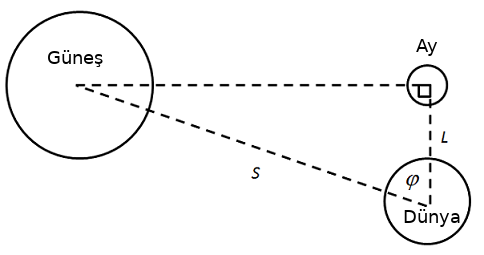
\includegraphics[width=20em]{sunmoon.png}

Yani ortaya bir dik üçgen çıkmış oldu. Bulmak istediğimiz $S/L$ oranı. Açı
$\varphi$ dünyadaki aletlerle ölçülebilir, kabaca aya doğru kolumuzu dik
uzatırız, sonra döndürüp güneye doğru işaret ettik diyelim, bu geçişin açısı
$\varphi$ açısıdır. Bu açıyı Aristarchus 97 derece olarak ölçtü. Dünya-Güney-Ay
üçlüsünün o andaki yerlerinin bir dik üçgenin köşeleri (çünkü yarım ay fazından
bu böyle olmalı). O zaman $S/L$ oranı nasıl bulunur?  $\varphi$ için kosinüs
hesabı $L/S$ değil midir?  Evet. O zaman bilinen $\varphi$'ın kosinüsünü ters
çevirirsek, istediğimiz orana erişiriz, $S/L = 1/(L/S) = 1 / \cos\varphi$,

\begin{minted}[fontsize=\footnotesize]{python}
print (1./np.cos(np.deg2rad(87)))
\end{minted}

\begin{verbatim}
19.10732260929735
\end{verbatim}

Yani güneş bize aydan yaklaşık 19 kat daha uzaktadır. Bunu sadece basit açılarla
hesaplayabilmiş olduk.

Dünyanın Yuvarlaklığı, ve Çevre Uzunluğu

Eratosten (Erotosthenes) MO 276 - MO 194 yıllarında yaşayan bilim adamıdır. Bir
gün birinden öğrendi ki yazın en uzun günü 21. Haziran'da daha güneyde olan
Syene şehrinde eğer yere bir çubuk dikilirse, saat 12'de çubuğun hiç gölgesi
olmuyor. Pitagor zamanından beri aslında dünyanın yuvarlak olabileceği
tahmin ediliyordu, Eratosten acaba aynı uzun yaz gününde daha kuzeyde olan
İskendiriye'de yere bir çubuk dikersem saat 12'de ne görürüm diye düşündü [2].

Bunu yaptı ve gördü ki ufak ta olsa bir gölge var. 

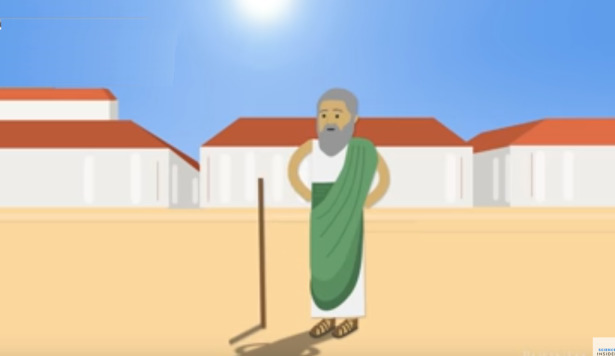
\includegraphics[width=20em]{circum3.jpg}

Sonra bu gölgenin sonuna kadar sopa basından doğru bir çizgi çekince, oluşan
açıya baktı,

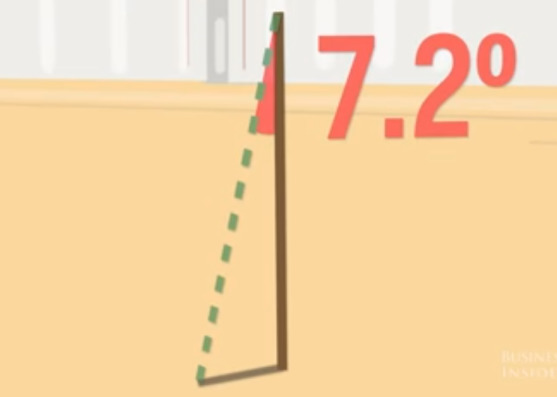
\includegraphics[width=20em]{circum4.jpg}

Bu önemli bir bilgiydi çünkü şimdi gökyüzüne düşen güneş ışınlarını düşünelim,
ışın öyle düşüyor ki o açı oluşmuş, 

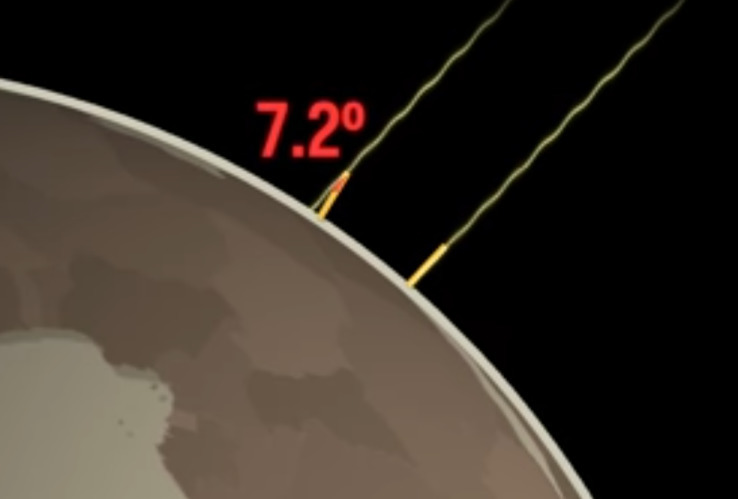
\includegraphics[width=20em]{circum1.jpg}

Şimdi bu ışını düz uzatırsak, bir de sopanın yönünde direk bir çizgiyi direk
dünya merkezine çekersek, bir üçgen ortaya çıkar, bir çizgiyi Syene şehrinin
sopasından direk dünya merkezine uzatabiliriz (bu çizgi direk merkeze gider
çünkü biliyoruz ki o anda oradaki sopanın gölgesi yok, güneş ışını direk sopanın
tepesine geliyor)

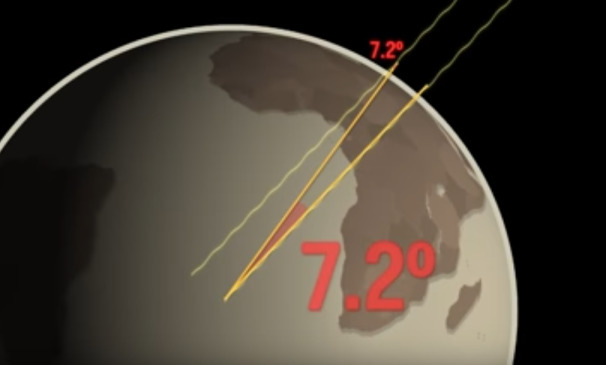
\includegraphics[width=20em]{circum2.jpg}

Böylece dünya merkezinden çıkan iki şehre doğru giden hayali iki çizginin
arasındaki açıyı bulmuş olduk. Bu açılar bize tam 360 dereceye göre bir oran
verir. Eh eğer İskenderiye ve Syene arasındaki gerçek yeryüzü mesafesini
buluyorsak bu oranla o mesafeyi çarpınca tüm dünyanın çevre uzunluğunu elde
edebiliriz. Eratosten birine yeryüzü mesafesini ölçtürdü, o kişi iki şehir
arasında yürüyerek bu ölçümü yaptı, bulduğu sonuç 5000 stadya, bugünkü
ölçüyle yaklaşık 800 km oluyor, oranla çarparsak,

\begin{minted}[fontsize=\footnotesize]{python}
print ('%0.2f km' % (360 / 7.2 * 800.0))
\end{minted}

\begin{verbatim}
40000.00 km
\end{verbatim}

Bu müthiş bir hesap, çünkü bugün daha kesin aletlerle yapılan ölçümlerin bulduğu
sonuç 40,075 kilometredir.

Kaynaklar

[1] Wikipedia,
    \url{https://en.wikipedia.org/wiki/On_the_Sizes_and_Distances_(Aristarchus)}

[2] Science Insider, {\em How The Ancient Greeks Proved Earth Wasn't Flat 2,200 Years Ago},
    \url{https://youtu.be/EfZ2HZH5CkA}
    
\end{document}


